\section{Numerical Optimization Approaches} \label{D. Numerical optimization approaches}
This category of algorithms describes the path planning problem as a cost function, which is then minimised by using function approximation techniques and machine learning methods.

\subsection{Potential Field Method}
The main concept of the Potential Field Method (PFM) \cite{gonzalez2016review, ge2002dynamic, barraquand1992numerical} algorithm is to fill the map with a potential field $f$ in which the robot is attracted towards the goal and repulsed from obstacles. The potential field $f$ is composed of two functions: $f = a + r$ where $a$ is the attraction function and $r$ is the repulsion function. After the potential function is computed, an optimisation technique of finding the minimum of $f$, such as gradient descent, is applied (See Figure \ref{fig:pfm}). The Wave-front Planner \ref{sec: wave-front} is an example of a potential function $f=a$ where the repulsion function is missing.

The space complexity is $\mathcal{O}(nm)$ where $n$ is the width and $m$ is the height of the map. The time complexity is $\mathcal{O}(\mathcal{O}(f) + \mathcal{O}(gradient\_descent))$. $\mathcal{O}(f) = \mathcal{O}(\mathcal{O}(a) + \mathcal{O}(r))$ depends on the choice of $a$ and $r$. Assuming same $a$ as in the Wave-front Planner, $\mathcal{O}(a) = \mathcal{O}(b^d)$, where $b$ is the branching factor and $d$ is the depth. Assuming that we use a simple $r$ which inflates the obstacle, the time complexity of $\mathcal{O}(r)$ is $\mathcal{O}(xo)$, where $x$ is the inflation rate and $o$ is the average obstacle size. $\mathcal{O}(gradient\_descent)$ is more involved if we use real gradient descent optimisation as it is based on the convergence rate. If we were to use the same gradient descent method from the Wave-front Planner, then $\mathcal{O}(gradient\_descent) = \mathcal{O}(d)$, where $d$ is the depth of the solution. The final time complexity is $\mathcal{O}(b^d + xo + d)$.

This solution is appealing because it is mathematically elegant and simple. It behaves well on complex environments which contain narrow passages, and it keeps a safe distance from the obstacles based on different factors such as relative velocity. Moreover, the algorithm can be extended to highly dynamic environments in which the obstacles and the goal are continually moving. Lastly, we can use vehicle parameters such as velocity and torque, to define $a$ and $r$. Thus, we can avoid collisions based on the velocity of the vehicle (i.e. when the vehicle has a high enough velocity to not being able to exit a collision trajectory) \cite{ge2002dynamic}.

One of the major drawbacks of using this method is that depending on the choice of $f$, local minimum problems might arise. Usually, these problems require particular solutions and rigorous analysis to ensure that there is no situation in which the agent will be trapped forever.

\begin{figure}[h!]
    \centering
    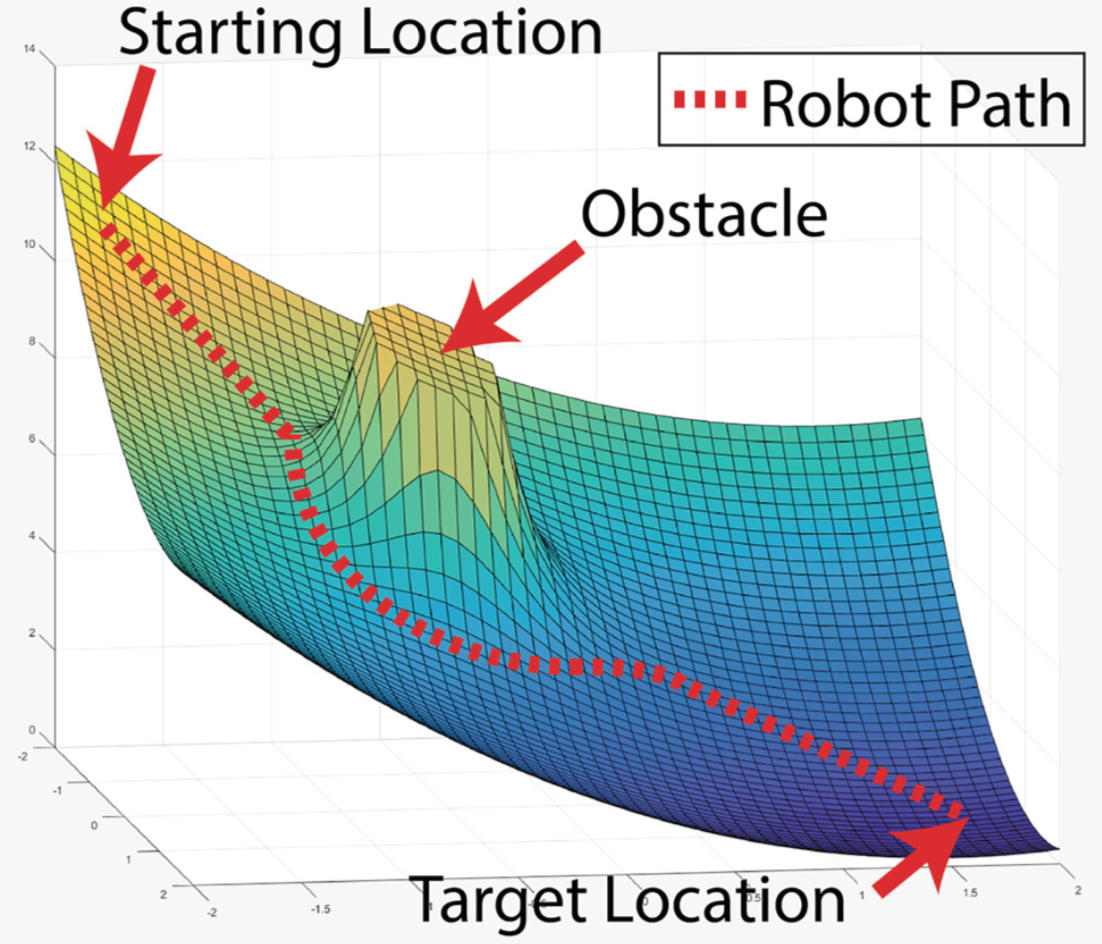
\includegraphics[scale=0.3]{images/pfm.png}
    \caption{Potential field $f = a + r$, where $a$ is the attraction function and $r$ is the repulsion function \cite{inproceedings}}
    \label{fig:pfm}
\end{figure}

\pagebreak

\subsection{LSTM}
Currently, the most important works that have considered LSTMs in this field are \cite{nicola2018lstm, lee2018lstm, inoue2019robot}.

%\cite{nicola2018lstm} uses an LSTM network to generate a path from the agent to the goal. The network was trained using A* on randomly generated maps and tested on maps from the online game Dragon Age. The issue with this approach is that the agent might get lost and will not succeed in finding a path to the goal, if there exists one. It has also been noticed that the algorithm has a higher success rate if the size of the map is relatively small and simple in layout.

Nicola et al. attempt to use an LSTM network to create an online global path planner by generating a low-resolution high-level path from start to goal \cite{nicola2018lstm}. The network was trained on randomly filled generated mazes with different corridor sizes with A* \ref{sec:a_star} as ground truth and tested on maps from the popular game Dragon Age. The primary motivation of using the proposed method from \cite{nicola2018lstm} is that, unlike A* which is offline (directly produces the final output), this method is an online search strategy that takes into account the fact that the environment is usually unknown or too expensive to store. Thus, at each time step, the network is queried for the next action that it should take given the local information of the map and previous choice of action. One of the significant drawbacks is that the rate of success of the algorithm gets lower as the map becomes more complicated (longer corridors, more complex objects).

Lee et al. make use of the LSTM architecture to extend the state of the art Value Iteration Networks (VIN) \cite{lee2018lstm}. VINs are similar to the Value Iteration algorithm described in \label{sec:vin} applied on a 2D grid world, but without making use of pre-defined MDP parameters such as the transition probabilities and rewards. The paper has pointed out that, despite being so successful, there are still issues with the current design of VIN such as the design of the transition model and the large number of recursive calls taken to achieve a reasonable estimate of the optimal path to the goal. The proposed solution replaces the recurrent VIN update rule with an LSTM kernel. \cite{lee2018lstm} has shown that the performance of the new solution has better or at least as good performance as the original VIN.

Inoue et al. aim to use a Convolutional Auto-encoder (CAE) combined with an LSTM to plan a path under a changing environment, by disregarding the unknown environment constraint (the map is fully discovered) \cite{inoue2019robot}. The two network sections are trained individually. Firstly, the CAE is trained on randomly generated maps with obstacles of different sizes. After that, the decoder is discarded, and the encoder is used to encode the same maps in order to extract the main features. Secondly, the LSTM is trained on the encoded maps by using RRT as ground truth. Unlike \cite{nicola2018lstm}, the solution is offline as it produces a full path (which might collide with obstacles), but it can be easily converted to an online solution in order to handle collision detection and prevention. A significant difference between this solution and \cite{nicola2018lstm} is that it has a higher overall success rate, which might arise since the CAE learns the input features as opposed to being hand crafted as in \cite{nicola2018lstm}.

%\cite{inoue2019robot} has a similar approach to \cite{nicola2018lstm}, but, in addition, it compares the LSTM network to a Value Iteration Network. The results show that the LSTM is, overall, better than the Value Iteration Network, but, still, they share the same issues as \cite{nicola2018lstm} (i.e. the algorithm has a low success rate of finding a path to the goal and if it finds one it is usually not optimal).


%\subsection{Machine Learning and Neural Networks methods}
%VIN (Value Iteration Networks)
%LSTMIN (Long Short Term Memory Iteration Networks)